\documentclass[a4paper,12pt]{article}
\usepackage[top = 2.5cm, bottom = 2.5cm, left = 2.5cm, right = 2.5cm]{geometry}
\usepackage[T1]{fontenc}
\usepackage[utf8]{inputenc}
\usepackage{multirow} 
\usepackage{booktabs} 
\usepackage{graphicx}
\usepackage[spanish]{babel}
\usepackage{setspace}
\setlength{\parindent}{0in}
\usepackage{float}
\usepackage{fancyhdr}
\usepackage{amsmath}
\usepackage{amssymb}
\usepackage{amsthm}
\usepackage[numbers]{natbib}
\newcommand\Mycite[1]{%
	\citeauthor{#1}~[\citeyear{#1}]}
\usepackage{graphicx}
\usepackage{subcaption}
\usepackage{booktabs}
\usepackage{etoolbox}
\usepackage{minibox}
\usepackage{hyperref}
\usepackage{xcolor}
\usepackage[skins]{tcolorbox}
%---------------------------

\newtcolorbox{cajita}[1][]{
	 #1
}

\newenvironment{sol}
{\renewcommand\qedsymbol{$\square$}\begin{proof}[\textbf{Solución.}]}
	{\end{proof}}

\newenvironment{dem}
{\renewcommand\qedsymbol{$\blacksquare$}\begin{proof}[\textbf{Demostración.}]}
	{\end{proof}}

\newtheorem{problema}{Problema}
\newtheorem{definicion}{Definición}
\newtheorem{ejemplo}{Ejemplo}
\newtheorem{teorema}{Teorema}
\newtheorem{corolario}{Corolario}[teorema]
\newtheorem{lema}[teorema]{Lema}
\newtheorem{prop}{Proposición}
\newtheorem*{nota}{\textbf{NOTA}}
\renewcommand\qedsymbol{$\blacksquare$}
\usepackage{svg}
\usepackage{tikz}
\usepackage[framemethod=default]{mdframed}
\global\mdfdefinestyle{exampledefault}{%
linecolor=lightgray,linewidth=1pt,%
leftmargin=1cm,rightmargin=1cm,
}




\newenvironment{noter}[1]{%
\mdfsetup{%
frametitle={\tikz\node[fill=white,rectangle,inner sep=0pt,outer sep=0pt]{#1};},
frametitleaboveskip=-0.5\ht\strutbox,
frametitlealignment=\raggedright
}%
\begin{mdframed}[style=exampledefault]
}{\end{mdframed}}
\newcommand{\linea}{\noindent\rule{\textwidth}{3pt}}
\newcommand{\linita}{\noindent\rule{\textwidth}{1pt}}

\AtBeginEnvironment{align}{\setcounter{equation}{0}}
\pagestyle{fancy}

\fancyhf{}









%----------------------------------------------------------
\lhead{\footnotesize Álgebra Moderna}
\rhead{\footnotesize  Rudik Roberto Rompich}
\cfoot{\footnotesize \thepage}


%--------------------------

\begin{document}
 \thispagestyle{empty} 
    \begin{tabular}{p{15.5cm}}
    \begin{tabbing}
    \textbf{Universidad del Valle de Guatemala} \\
    Departamento de Matemática\\
    Licenciatura en Matemática Aplicada\\\\
   \textbf{Estudiante:} Rudik Roberto Rompich\\
   \textbf{Correo:}  \href{mailto:rom19857@uvg.edu.gt}{rom19857@uvg.edu.gt}\\
   \textbf{Carné:} 19857
    \end{tabbing}
    \begin{center}
        MM2035 - Álgebra Moderna - Catedrático: Ricardo Barrientos\\
        \today
    \end{center}\\
    \hline
    \\
    \end{tabular} 
    \vspace*{0.3cm} 
    \begin{center} 
    {\Large \bf  Tarea 13
} 
        \vspace{2mm}
    \end{center}
    \vspace{0.4cm}
%--------------------------


\section{Estados financieros}

\subsection{Estado de resultados}
    Provee información acerca de las operaciones de un negocio, al igual que sus 
eficiencias a distintos niveles según se analice. 

\begin{itemize}
    \item Ingresos (ventas) 
    \item Costo de Materias Primas | Gastos de Producción (costos) 
    \item Margen de Ventas (utilidad bruta) 
    \item Gastos  de;  Mano  de  Obra,  Administrativos,  Depreciación,  Marketing, 
    Operacionales, Alquileres, IVA por Pagar etc. (gastos operativos) 
    \item Gastos de Intereses (gastos financieros) 
    \item Pago de Impuestos (impuestos) 
    \item Ganancias Netas (utilidad neta)
\end{itemize}


\begin{figure}[H]
    \centering
    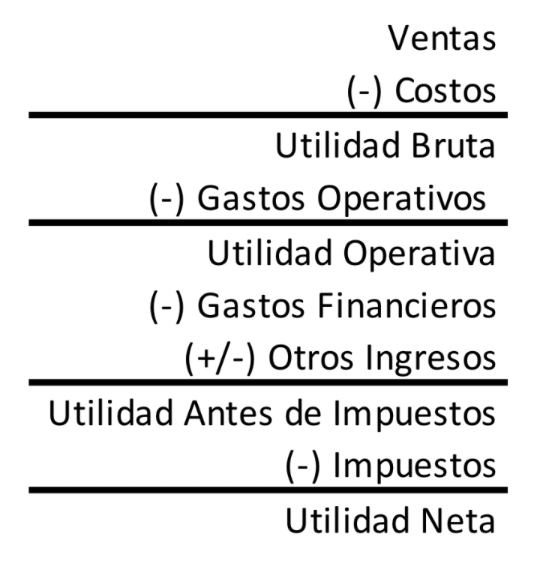
\includegraphics[scale=0.5]{imagenes/1.1.png}
\end{figure}





\subsection{Balance general}
    Provee información acerca del valor real o teórico, de todos los bienes y 
obligaciones de una empresa, en un período determinado. Valor  de  libros  de  los  bienes,  obligaciones  y  capital  de  los  accionistas  de  una 
empresa. 

$$\text{Activos} = \text{Pasivos} +\text{Capital}$$

\subsubsection{Corto Plazo o Circulantes}

\begin{itemize}
    \item Todo  lo  que  pueda  ser  convertido  en  efectivo  en  el  transcurso  de  un  año,  u  
    obligación que tenga que ser pagada en el próximo año. 
    \item El corto plazo y la liquidez de una compañía están correlacionados. 
    $$\text{Razón Corriente} = \frac{Activos Corrientes}{Pasivos Corrientes} $$
\end{itemize}

\subsubsection{Largo Plazo o No Circulantes }
Todo  lo  que  pueda  ser  convertido  en  efectivo,  u    obligación  que  tenga  que  ser 
pagada de 1 año en adelante. 
Tangibles 

\subsubsection{Tangibles}
Activos con forma física, pueden ser a corto plazo o largo plazo. 
Intangibles.

\subsubsection{Intangibles}
Marcas, Patentes, Goodwill, Licencias de Uso, Reconocimiento de Marca, etc

\begin{figure}[H]
    \centering
    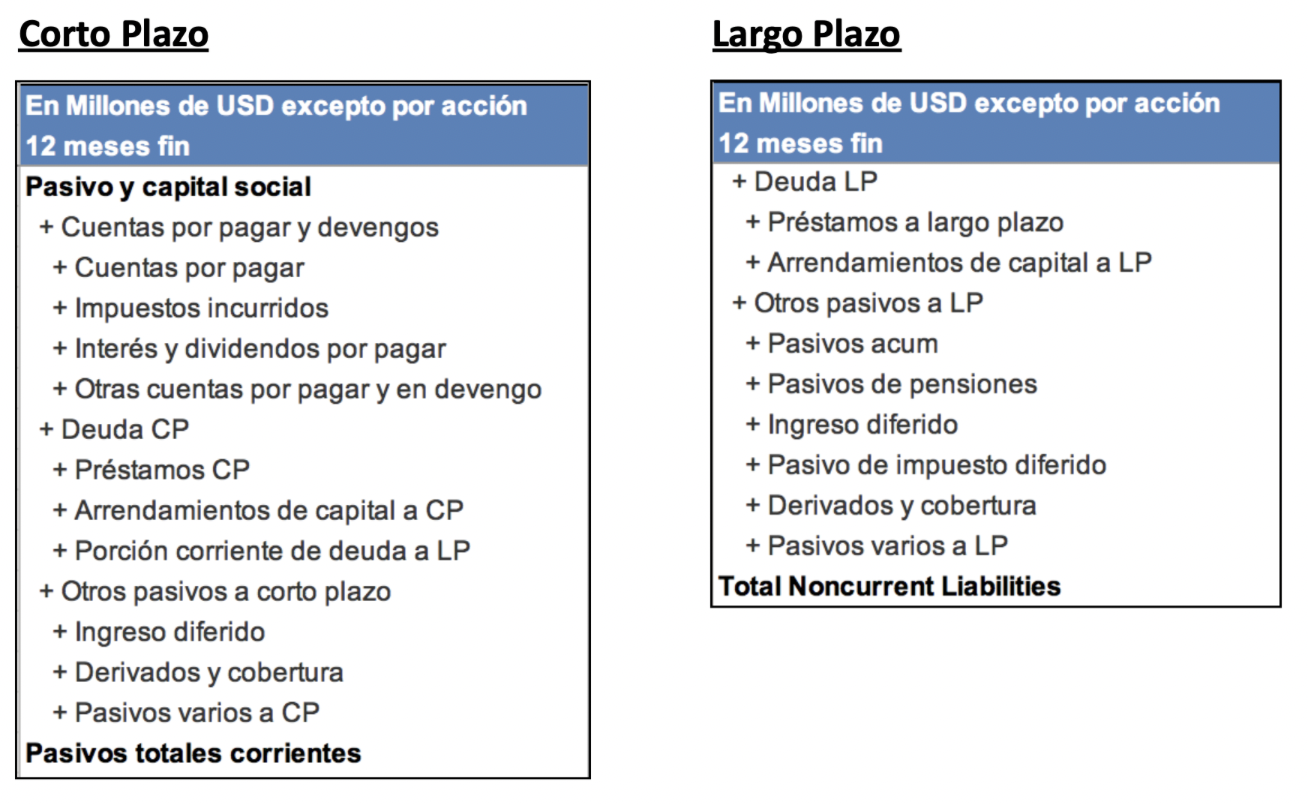
\includegraphics[scale=0.3]{imagenes/1.2.png}
\end{figure}

\begin{figure}[H]
    \centering
    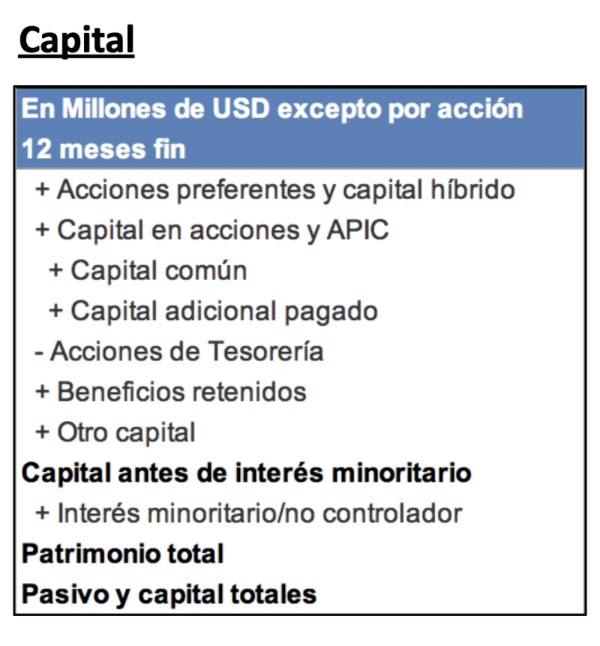
\includegraphics[scale=0.3]{imagenes/1.3.png}
\end{figure}

\begin{itemize}
    \item A  partir  del  Balance  General  podemos  estimar  el  \textbf{Valor en Libros}  de  una compañía. Es  valor  de  una  compañía|activo,  si  dejara  de  operar  en  este  momento vendiendo todos sus activos y pagará todas sus deudas. Se calcula sumando todos los activos tangibles, y quitando los pasivos: 
    $$\text{Valor en Libros} = \text{Activos Tangibles} - \text{Pasivos} $$
    Es  el  valor  contable,  no  necesariamente  refleja  el  valor  de  mercado  del activo  o  empresa  en  sí.  Es  un  acercamiento  para  el  valor  mínimo  de  una compañía o empresa. Se asume como si la empresa dejara de opera
\end{itemize}




\subsection{Flujo de caja}
    Provee la información acerca de los ingresos y egresos de la operación 
de la compañía (giro de negocio), la compra y venta de activos, y las 
obligaciones o ingresos de deudas financieras.

\subsubsection{Utilidad Neta} 
    Se  inicia  el  Flujo  Operativo  con  la  Utilidad  Neta,  ya  que  está  refleja  el 
resultado final de la operación. 
\subsubsection{Cuentas por Cobrar (CxC)}
    Los aumentos son negativos, ya que representan ingresos del Estado de 
Resultados,  en  ventas,  que  nunca  fueron  ingresos  de  efectivo.  Los 
decrementos son positivos, ya que representan pagos de los clientes. 
\subsubsection{Inventario}
    Los aumentos indican que la compañía produjo/compro, más bienes de los 
que vendió, por lo tanto es una salida de efectivo adicional. La disminución, 
indica que la compañía utilizó los materiales ya existentes.

\subsubsection{Cuentas por Pagar (CxP) y/o Depreciación}
    Los aumentos son positivos, ya que son gastos "incurridos" que no son reales hasta que son pagados. Cuando disminuyen es por qué fueron pagados. 
\subsubsection{Cambio en Fijos e Intangibles (CAPEX) [parte de Flujo de Inversión]}
    Cualquier  inversión  en  activos  fijos;  Propiedad,  Planta  y  Equipos  (aumentos) representa  un  gasto  el  cual  no  es  reflejado  en  el  estado  de  resultados.   
    Cualquier  venta  de  activos  fijos;  Propiedad,  Planta  y  Equipos  (disposición/disminución),  representa  un  ingreso  que  no  se  refleja  en  el  estado  de 
resultados. 
\subsubsection{Cambios en Deuda [parte de Flujo Financiero]}
    La adquisición de deuda representa un aumento efectivo, mientras que el pago de deuda representa una disminución.

\subsubsection{Efectos de Tipo Cambiario (Effect of Foreign Exchange Rates)}
    Si la empresa recibe divisas (monedas) diferentes a la de la Casa Matriz, se  debe  de  reflejar  cualquier  pérdida  o  ganancia  si  el  tipo  de  cambio aumenta o disminuye.

    \begin{figure}[H]
        \centering
        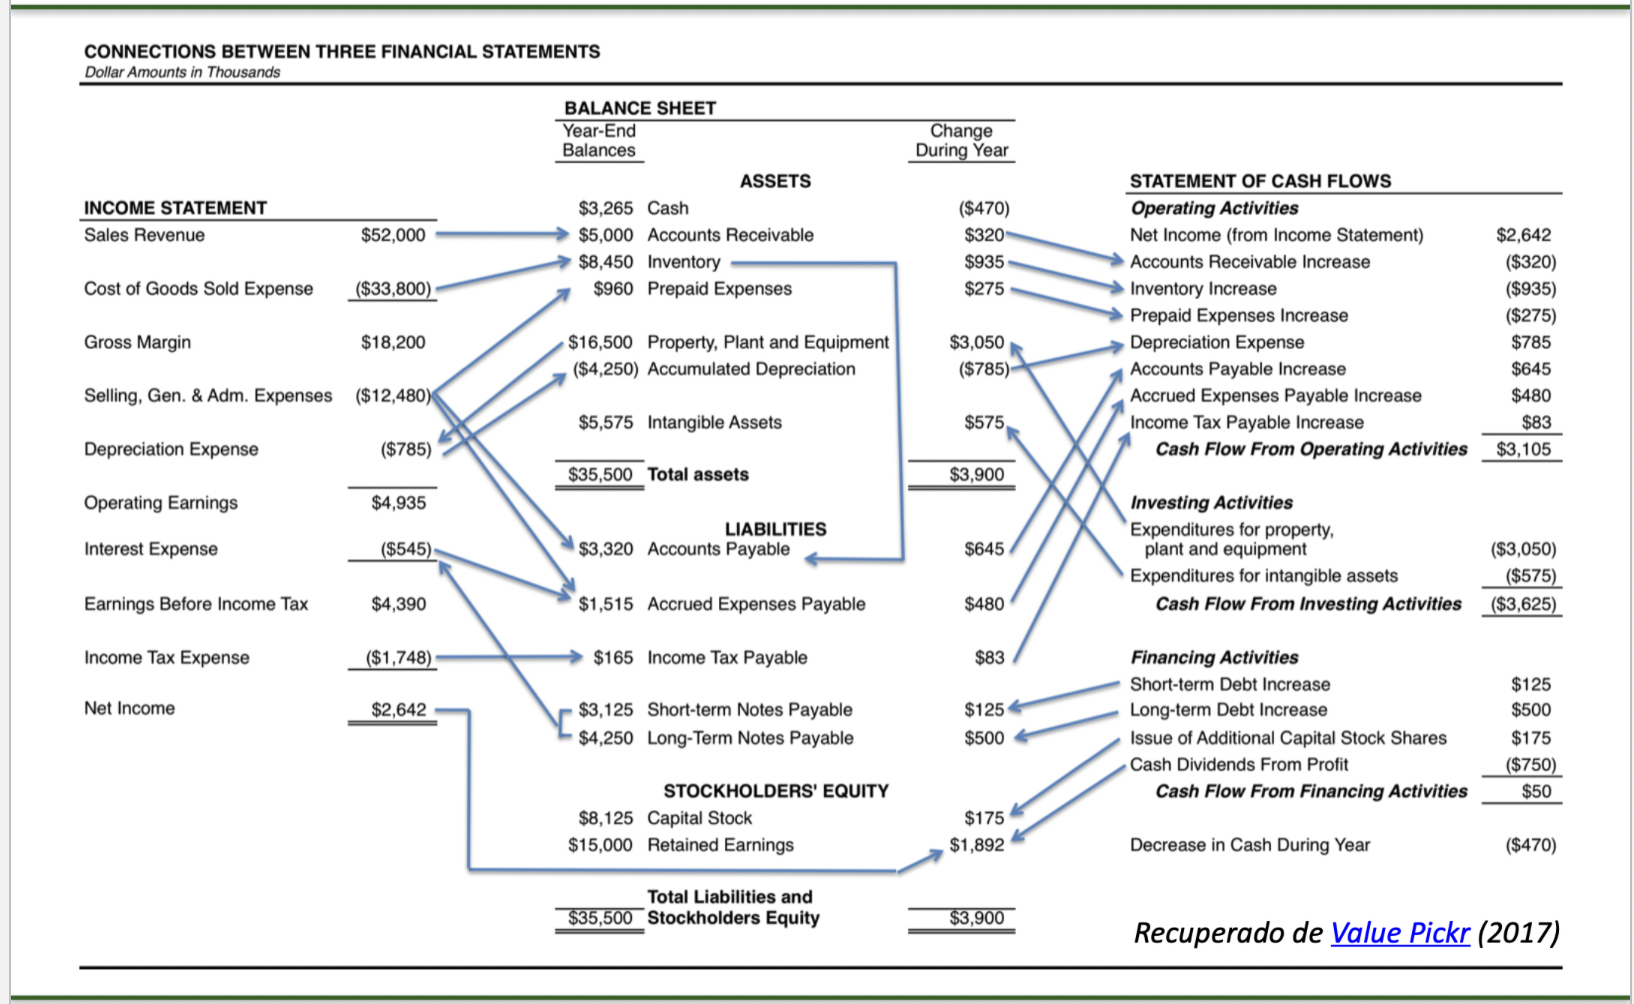
\includegraphics[scale=0.3]{imagenes/1.png}
    \end{figure}
    
    



    \begin{cajita}
        \begin{itemize}
            \item Estado de resultados. 
            \begin{itemize}
                \item Operación del giro de negocio: 
                \begin{enumerate}
                    \item Rendimiento de ventas
                    \item Costos y gastos principales 
                    \item Pago de Impuestos
                \end{enumerate}
            \end{itemize}
            \item Balance general 
            \begin{itemize}
                \item Manejo de bienes y de obligaciones en el corto y largo plazo: 
                \begin{enumerate}
                    \item Registro de lo que le pertenece y lo que debe la empresa y sus accionistas. 
                    \item Igualdad (ecuación contable)
                \end{enumerate}
            \end{itemize}
            \item Flujo de caja
            \begin{itemize}
                \item Entradas y salidas reales de efectivo: 
                \begin{enumerate}
                    \item Efectivo del giro de negocio
                    \item Efectivo del manejo de activos (inversión = activos)
                    \item Efectivo del manejo de deudas, pago de dividendos o compra y emisión de acciones.
                    \item Requiere de cuentas del E.R y B.G. 
                \end{enumerate}
            \end{itemize}
        \end{itemize}
    \end{cajita}
    

\section{Razones financieras}

\subsection{Razón corriente}

\begin{itemize}
    \item Mide  la  capacidad  de  la  empresa  para  hacer  frente  a  sus  pagos  de  corto  plazo,  y  está 
    directamente ligado a la liquidez de la empresa. 
    \item Cálculo 
        $$\text{Razón Corriente} =\frac{\text{Activos Corrientes}}{\text{Pasivos Corrientes}} $$
    \item Si es mayor a 1, la empresa puede cubrir todas sus obligaciones (pagos) a corto plazo. Si es 
    menor a 1, la empresa tendrá problemas o no podrá cubrir el total de las obligaciones a corto 
    plazo. Generalmente una razón corriente elevada (mayor a uno) es deseada.
    \item Se  asume  que  se  pueden  liquidar  el  100\%  de  los  activos  corrientes,  no  considera  la 
    composición de los AC (Rotación CxC, Inventario, Inversiones de Corto Plazo).
\end{itemize}


\subsection{Prueba ácida}

\begin{itemize}
    \item Mide  la  capacidad  de  la  empresa  para  hacer  frente  a  sus  pagos  de  corto  plazo,  eliminando  el 
    inventario bajo la premisa que no será posible venderlo. 
    \item Cálculo 
    {\small$$\text{Prueba Ácida Rápida} = \frac{\text{Activos Corrientes - Inventarios}}{\text{Pasivos Corrientes}} $$}

    {\small$$\text{Prueba Ácida Extendida} =  \frac{\text{Efectivo + Inversiones Corto Plazo + Cuentas por Cobrar (corto plazo)}}{\text{Pasivos Corrientes}} $$}
                                                        
    \item Si es mayor a 1, la empresa puede cubrir todas sus obligaciones (pagos) a corto plazo. Si es menor a 
    1,  la  empresa  tendrá  problemas  o  no  podrá  cubrir  el  total  de  las  obligaciones  a  corto  plazo. 
    Generalmente una prueba ácida elevada (mayor a uno) es deseada. 
    \item Gastos|Servicios pagados por anticipado, no considera el inventario el cual generalmente no es fácil 
    de convertir a efectivo, aunque existen excepciones (Au).
\end{itemize}




\subsection{Ciclo de conversión de efectivo}

\begin{itemize}
    
\item Mide el tiempo en que una la empresa vende su inventario, cobra sus cuentas y paga sus cuentas. 
 
\item Tenemos: 
\begin{itemize}
\item 
     Ciclo de Conversión de Efectivo =  RID + RCxCD - RCxPD 
\item 
     RID = Rotación Inventarios en Días = (Inventario Promedio / Costo de Ventas) * 365 
\item 
     RCxCD = Días de CxC = (Cuentas por Cobrar Promedio / Ventas Netas)* 365 
\item 
     RCxPD = Días de CxP = (Cuentas por Pagar Promedio / Costo de Ventas) * 365

\end{itemize}
 
\item Entre más pequeño sea el ciclo, la empresa es más líquida. Si el ciclo es negativo, la empresa tiene 
paga en más tiempo del que tiene los productos. 
Observaciones 
\item Presenta una ventaja sobre la prueba ácida extendida, ya que permite medir la liquidez en términos de 
tiempo.
\end{itemize}


\subsection{Razones de apalancamiento}
\begin{itemize}
    \item  Mide el porcentaje que representa todos los pasivos en relación a los activos totales, es el riesgo al 
    cual está expuesta en términos de obligaciones. 
    \item Cálculo 
    \begin{itemize}
        \item Apalancamiento  =   Pasivos Totales / Activos Totales
        \item Deuda (Préstamos) a Activos =  Préstamos Totales /  
        Activos Totales 
    \end{itemize}

    \item Un  valor  pequeño  (menor  a  0.50)  de  significa  que  hay  menos  apalancamiento  (utiliza  más 
    Patrimonio de los Accionistas, en vez de deuda). En el caso de Deuda a Activos, mide la proporción 
    de la deuda con la cual se han adquirido activos, como ha utilizado el dinero prestado. 
     
    \item No necesariamente entre menor o mayor sea esta razón, será siempre mejor, dependerá de cada 
    industria. El valor de esta siempre será menor a 1
\end{itemize}

\subsection{Razones de apalancamiento}

\begin{itemize}
    \item Mide  la  relación  de  la  posición  de  cuánto  han  aportado  los  acreedores  versus  los 
    accionistas. 
    \item Cálculo 
    \begin{itemize}
        \item Pasivos a Patrimonio =  Pasivos Totales/Patrimonio Total
        \item  Deuda (Préstamos) a Patrimonio =  Préstamos Totales/Patrimonio Total 
    \end{itemize}
 
   \item Un valor pequeño significa que los accionistas han aportado más a la empresa, por lo cual hay menos apalancamiento. 
    \item No necesariamente entre menor o mayor sea está razón, será siempre mejor.
\end{itemize}

\subsection{Cobertura de interés}
\begin{itemize}
    \item  Mide la capacidad de hacerle frente al gasto de la deuda, el interés, en relación a la capacidad operativa para generar ingresos, con la utilidad antes impuestos. 
    \item Cálculo 
    \begin{itemize}
        \item Cobertura de Interés =  Utilidad Antes de Impuestos / Gasto de Interés 
    \end{itemize}
    
    \item Entre mayor sea este multiplicador, la empresa tiene más recursos operativos 
    para pagar proporción del período respecto préstamos totales adquiridos. 
    \item Únicamente se observa el Estados de Resultados.
\end{itemize}
\subsection{Razón de cobertura}
\begin{itemize}
    \item  Mide la capacidad de hacerle frente a la deuda total, respecto al flujo de efectivo que genera una empresa con sus operaciones. 
    \item Cálculo 
    \begin{itemize}
        \item Razón de Cobertura =  Flujo de Caja Operativo/Préstamos Totales
    \end{itemize}
    \item Entre mayor sea este multiplicador, la empresa tiene más efectivo operativo real para 
    pagar los préstamos totales adquiridos para la misma. 
    \item Proporciona una vista global real respecto al pago de los préstamos (la cobertura de 
    interés habla del gasto de los préstamos).
\end{itemize}

\subsection{Rotación de activos}

\begin{itemize}
    \item  Mide la eficiencia en el uso de los activos para genera ventas. 
    \item Cálculo 
    \begin{itemize}
        \item Rotación de Activos = Ventas Netas/ Activos Totales Promedio 
    \end{itemize}
    \item Entre mayor sea este multiplicador, la empresa tiene es más eficiente en el uso de sus activos, sus activos rinden más. 
    \item Los activos totales incluyen todas las cuentas, es difícil de identificar o atribuir 
    directamente la cuenta que contribuye más a las ventas para darle seguimiento.
\end{itemize}
\subsection{Rentabilidad}
\begin{itemize}
    \item  Mide  la  eficiencia  en  el  uso  del  recursos  (costos  y  gastos),  respecto  a  las  ventas  para  crear  valor  a  la 
    empresa. 
    \item Cálculos 
    \begin{itemize}
        \item Margen Bruto =  Utilidad Bruta/Ventas Netas 
        \item Margen Operativo =  Utilidad Operativa/ Ventas Netas 
        \item Margen Antes de Imp. =  Utilidad Antes de Impuestos / Ventas Netas 
        \item  Margen Neto =  Utilidad Neta/Ventas Netas 
    \end{itemize}
 
    \item Entre mayor sea este número, la empresa es más rentable. 
    Observaciones 
    \item Cada margen mide la rentabilidad en distintos punto del ER, cada uno es valioso para hallar oportunidades.
\end{itemize}
\subsection{Rentabilidad}
\begin{itemize}
    \item Mide la eficiencia en el uso del recurso humano para generar ventas. 
    \item Cálculo 
    \begin{itemize}
        \item Ventas por Empleado = Ventas Netas/Empleados Totales 
    \end{itemize}
    \item Entre mayor sea este número, la empresa es más eficiente en el uso de sus recursos humanos. 
    \item Es  relevante  comparar  con  la  competencia  y  tener  clara  la  proporción  de personal operativo vs personal administrativo.
\end{itemize}

\subsection{Rentabilidad}

\begin{itemize}
    \item Mide capacidad de una empresa para convertir sus ventas a efectivo. 
    \item Cálculo 
    \begin{itemize}
        \item Flujo Operativo a Ventas =  Flujo de Caja Operativo / Ventas Netas Totales 
    \end{itemize}
    \item Si es positivo la empresa es capaz de generar efectivo con sus operaciones. Se desea que sea tan grande como se pueda. 
    \item Es una medida más real de generación de efectivo vs la Utilidad Neta.
\end{itemize}

\subsection{Rentabilidad}

\begin{itemize}
    \item  Mide la proporción del flujo neto que proviene de las operaciones de la empresa. 
    \item Cálculo 
    \begin{itemize}
        \item Flujo de Efectivo Neto a Flujo Operativo = Flujo de Efectivo Neto / Flujo de Caja Operativo 
    \end{itemize}

    \item Entre mayor sea este, representa una robustez financiera mayor en términos de generación de efectivo, con el cuidado que debemos de conocer la composición del flujo de efectivo neto. 
     
    \item Es  la  medida  más  real  de  solidez  financiera,  en  términos  de  generación  de efectivo real.
\end{itemize}


\subsection{Retorno sobre activos}

\begin{itemize}
    \item Mide  eficiencia  en  la  administración  para  generar  beneficios  para  la  empresa,  con  base  a  los 
    activos. 
    \item Cálculo 
    \begin{itemize}
        \item Retorno sobre Activos = Utilidad Neta/ Activos Totales Promedio
        \item Retorno sobre Activos de dos Pasos =  Margen Neto  *      Rotación de Activos 
        \item Retorno sobre Activos de dos Pasos =  (Utilidad Neta)/(Ventas Netas)  * 
       (Ventas Netas)/ (Activos Totales Promedio )
    \end{itemize}

    \item Entre más grande sea la razón, mejor administrados son los activos. 
    Observaciones 
    \item Los activos totales incluyen todas las cuentas, es difícil de identificar o atribuir directamente la 
    cuenta que contribuye más a las ventas para darle seguimiento.
\end{itemize}

\subsection{Retorno sobre inversión/capital}

\begin{itemize}
    \item Mide qué tanto ganan lo accionistas respecto al dinero invertido en la misma. 
    \item Cálculo
    \begin{itemize}
        \item Retorno sobre Capital (Patrimonio) = Utilidad Neta/Patrimonio Total Promedio 
        \item Dupont =  Margen Neto  * Rotación de Activos * Multiplicador de Capital 
        \item Dupont =  (Utilidad Neta)/(Ventas Netas) * (Ventas Netas)/(Activos Totales Promedio) * (Activos Totales Promedio)/(      Patrimonio Total Promedio) 
    \end{itemize}
    \item Entre más grande, la empresa está siendo administrada eficientemente y los accionistas están obteniendo mayores retornos. 
 
\item Es una medida más real de generación de efectivo vs la Utilidad Neta.
\end{itemize}


\section{Análisis vertical y horizontal}

\subsection{Análisis vertical}

\begin{itemize}
    \item Mide la proporción que representa cada una de las cuentas de un estado 
    financiero respecto a un criterio fijo (Ventas para Estado de Resultados, Activos Totales 
    para Balance General). 
    \item Es útil para identificar oportunidades de optimización de costos, gastos y 
    activos, y/o problemas con el manejo de los mismos. 
    \item Vale la pena comparar período con período para tener más información. 
\end{itemize}
\begin{figure}[H]
    \centering
    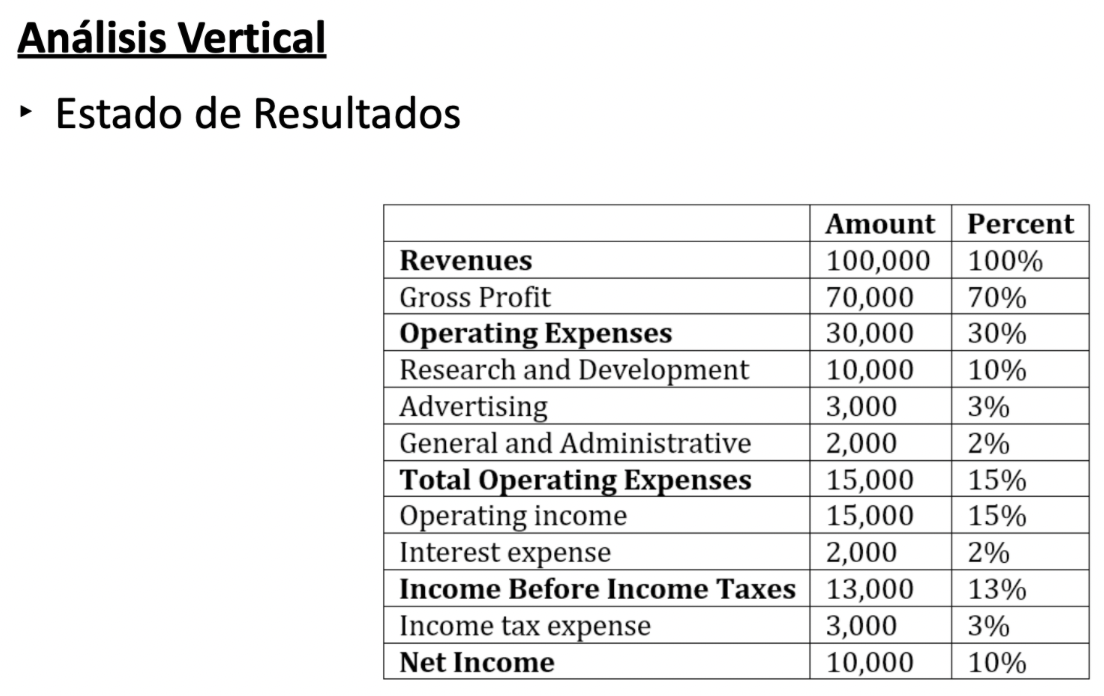
\includegraphics[scale=0.4]{imagenes/3.1.png}
\end{figure}

\begin{figure}[H]
    \centering
    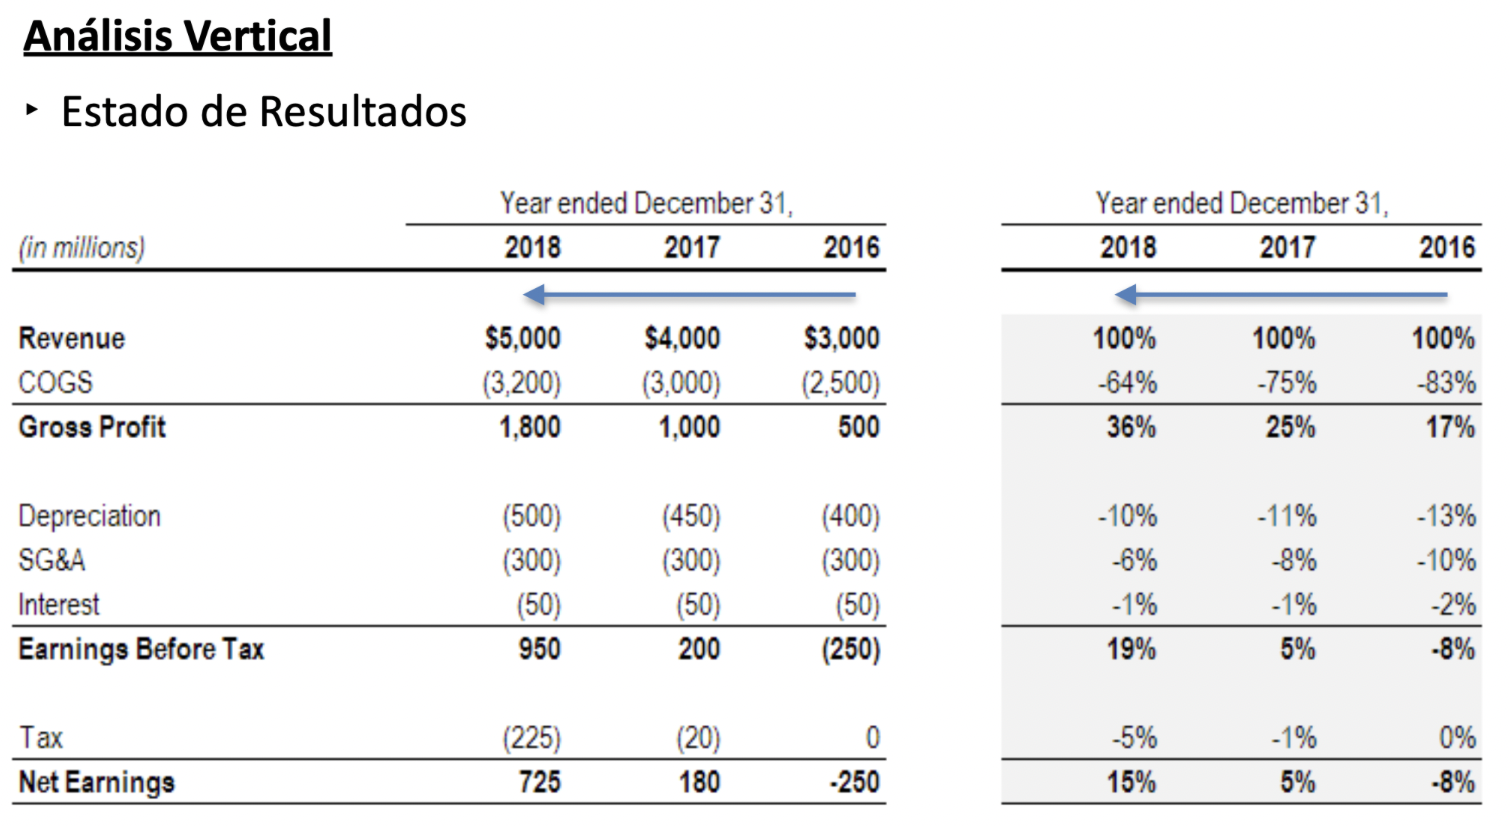
\includegraphics[scale=0.3]{imagenes/3.2.png}
\end{figure}

\begin{figure}[H]
    \centering
    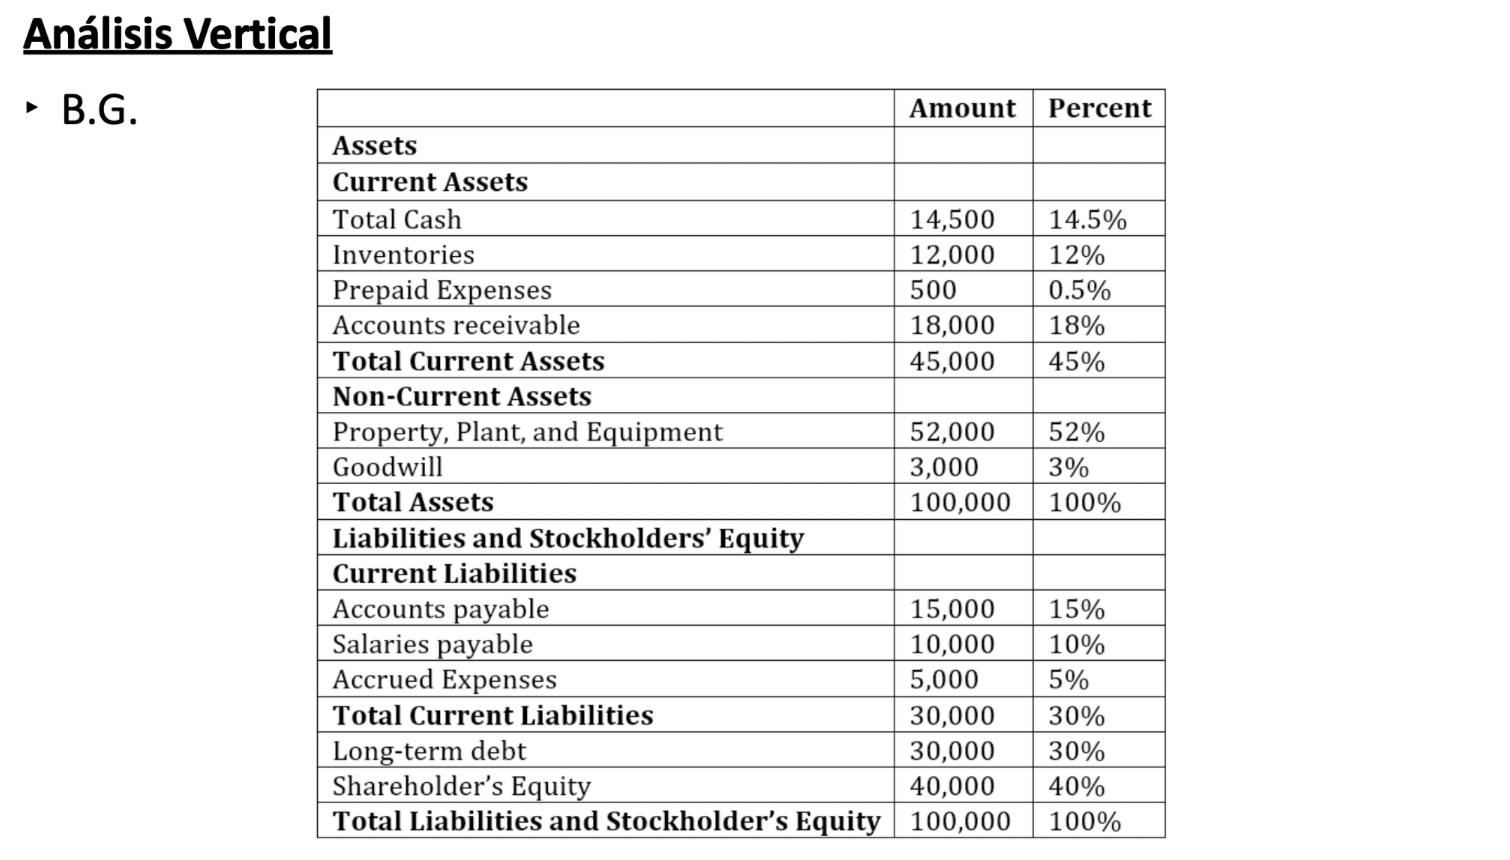
\includegraphics[scale=0.3]{imagenes/3.3.png}
\end{figure}



\subsection{Análisis horizontal}
\begin{itemize}
    \item Mide la evolución de crecimientos período con período, respecto a una misma cuenta. 
    \item Se  puede  hacer  indexado,  pero  provee  más  información  cuando  se 
    realiza período con período (D2D, M2M, Y2Y).
\end{itemize}

\begin{figure}[H]
    \centering
    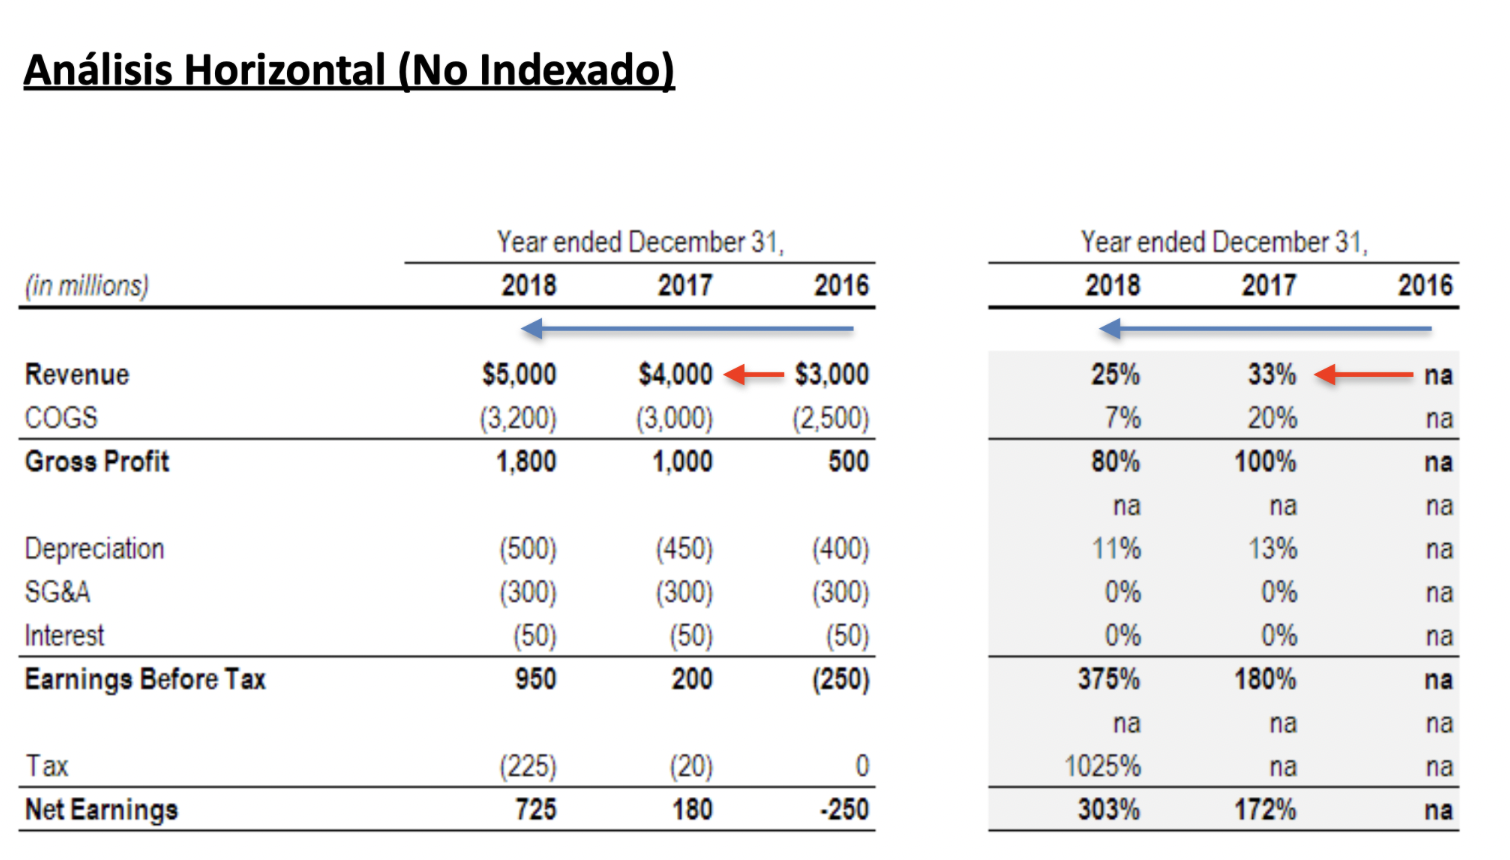
\includegraphics[scale=0.3]{imagenes/3.4.png}
\end{figure}


%---------------------------
%\bibliographystyle{apa}
%\bibliography{referencias.bib}

\end{document}